\chapter{Improving flexibility of macros}\label{sect:flex}
\label{improving-flexibility-macros}

% \todo[inline]{Explain the old macro system with an example. Q: Isn't that the section below already?}

% \section{Explanation of the macro system}
\section{The macro system}
% What are the limitations without macros?
% Most importantly: syncats. gf-ud assumes that every word is in a leaf, represented by a lexical gf-function. however, syncategorimatic words \todo{define?} (or functions?) come from the functions that are used to combine trees (what are those called?) and would be missing otherwise. E.g. "is" is syncategorimatic in gf for english, because there is no lexical function for copula, because not all languages use a word for copula. So we make up a lexical gf-function for "is", which is then combined with a made-up version of MkCl which is converted into the thing we need.
% This is terrible writing!

% Motivate need for auxfuns and auxcats

GF trees are on a higher abstraction level than UD trees. In UD, every token is associated with a dependency label. In contrast, any production rule in a GF grammar may introduce new tokens. This difference complicates the mapping between the two formalisms.

In order to overcome some limitations of the conversion from UD to GF, especially the issue with multiple possible matching trees mentioned in \autoref{sec:multiple_trees}, there is a system of macros. A macro is an imaginary GF function that will get converted into an expression of real GF functions after the main conversion step of gf2ud is done.

The full syntax of macros can be found in \autoref{app:annotation}.

% Syncats?
% \todo[inline]{Talk about syncategorematic words}
\subsection{Simple example: \texttt{\#auxfun} and matching morphological features}

When one GF function corresponds to multiple different dependency labels, a macro can be used to disambiguate which one is meant and to avoid losing the information of that distinction.

For example, if we have a noun without a determiner, the algorithm would try all possible ways to build a noun phrase out of it: an indefinite plural, using \verb|DetCN aPl_Det : CN -> NP|, or mass noun, using \verb|MassNP : CN -> NP|. But for a human reader it is obvious, because we know it from the form of the word: \emph{water} in ``I drink \emph{water}'' is a singular mass noun, and \emph{children} in ``\emph{Children} are playing'' is an indefinite plural.

The annotation scheme introduced in \autoref{sec:annotations-intro} operates on abstract syntax only, and thus it has no way to distinguish between those cases, because it has no information about concrete morphological features.
% In order to create mass noun phrases of singular nouns and plural noun phrases of plural nouns,

In order to choose the right function depending on features beyond the dependency label, the macros can also match against part of speech and morphological features using the syntax \verb|dependency_label[Feature=Value]|.

\begin{lstlisting}
    -- disable plurals as mass terms
    #disable MassNP aPl_Det
    #auxfun MassNP_sg cn : CN -> NP = MassNP        cn ; head[Number=Sing]
    #auxfun DetCN_aPl cn : CN -> NP = DetCN aPl_Det cn ; head[Number=Plur]
\end{lstlisting}

In order to use the macros instead of the original function, we first \verb|#disable| the original functions.
Next we create macros that check for the correct number before constructing.
Notice that the macro \verb|DetCN_aPl| combines the syntactic function \verb|DetCN : Det -> CN -> NP| with the lexical function \verb|aPl_Det : Det|.

Let's consider the sentence ``Children are playing'', and what would happen to it if we didn't force mass nouns and indefinite plurals to be introduced via macros.

The algorithm from \autoref{sec:overview-of-algorithm} goes through each word\footnote{Remember that all the words are parsed into a lexical category, which is determined by the \texttt{\#cat} annotation.}, and tries all possible functions that can be applied to them. If we have available \verb|MassNP : CN -> NP|, that tree is built every single time we have a CN available.
If the original phrase had a determiner, like ``Many children are playing'', then the NP formed by \verb|MassNP| is discarded as soon as the algorithm enters the next step and tries to combine the noun and the determiner.
But now that the phrase has no determiner in the first place, the algorithm could pick the \verb|MassNP| version, instead of the correct indefinite plural. And in fact, the algorithm would never build the correct \verb|DetCN aPl_Det| form without this macro, because the lexical function \verb|aPl_Det| does not correspond to any word, so it was never introduced into the tree.

\subsection{Complex example: \texttt{\#auxcat} and syncategorematic words}

Another common case when macros are needed are so-called \emph{syncategorematic} words, that are associated with non-lexical functions\footnote{A lexical function is a function that takes zero arguments, which means that it will be in a leaf of the tree.}. For example, in GF, the copula and many auxiliary words are syncategorematic, which means that they cannot be parsed on their own using GF.

The following is an example from \cite{kolachina-ranta-2017} that uses macros to handle the syncategorematic nature of the auxiliary verb \emph{have}:

\todo[inline]{Include some of the commented out content}

% We noted in Section 2 that ud2gf has to deal with
% ambiguity, incompleteness, noise, and ungrammaticality. The basic algorithm of Section 3 takes
% none of these aspects into account. But it does
% contain what is needed for ambiguity: the list ts
% of previous trees at each node can also be used
% more generally for storing alternative trees. The
% “main” tree t is then compared and ranked together with these candidates. Ranking based on
% tree probabilities in previous GF treebanks, as in
% (Angelov, 2011), is readily available. But an even
% more important criterion is the node coverage of
% the tree. This means penalizing heavily those trees
% that don’t cover all nodes in the subtrees.
% This leads us to the problem of incompleteness:
% what happens if the application of all possible candidate functions and trees still does not lead to a
% tree covering all nodes? An important part of this
% problem is due to syncategorematic words. For
% instance, the copula in GF is usually introduced as
% a part of the linearization, and does not have a category or function of its own.6 To take the simplest
% possible example, consider the adjectival predication function and its linearization:
% fun UseAP : AP -> VP
% lin UseAP ap = \\agr => be agr ++ ap
% where the agreement feature of the verb phrase is
% passed to an auxiliary function be, which produces
% the correct form of the copula when the subject
% is added. The sentence the cat is black has the
% following tree obtained from UD:





% \begin{verbatim}
% #auxfun MkVPS_Perf have vp : Have -> VP -> VPS = MkVPS (TTAnt TPres
%   AAnter) PPos vp ; aux[Tense=Pres] head
% \end{verbatim}


When introducing the problem and its partial solution, \cite{kolachina-ranta-2017} name as examples copulas, negations, tense auxiliaries and infinitive marks. We reproduce their example of the English copula (the verb “to be”) and its treatment in \verb|ud2gf|.

Figures \ref{fig:gf_cute} and \ref{fig:ud_cute} show the difference between GF’s and UD’s treatment of copulas. In the UD tree, the copula has a category and a dependency label \verb|cop|. In the GF tree, there is no special category: the string “is” is introduced by the function \verb|UseComp : AP -> VP| rule, which makes an AP into a predicate.

% \begin{figure}
%     \centering
%     \includegraphics{}
%     \caption{Caption}
%     \label{fig:enter-label}
% \end{figure}

% result from \verb+p -cat=Cl "this cat is small"  | vp -view=open -showfun+:

% Produced using: https://maryszmary.github.io/ud-annotatrix//standalone/annotator.html
% And pressing the printer icon to select latex

\begin{figure}
    \centering
    % \includegraphics{}
    \begin{dependency}
       \begin{deptext}[column sep=0.4cm]
             this \& cat \& is \& small \\
           {\tt DET}\&{\tt NOUN}\&{\tt AUX}\&{\tt ADJ}\\
       \end{deptext}
       \depedge{2}{1}{det}
       \depedge{4}{2}{nsubj}
       \depedge{4}{3}{cop}
    \end{dependency} \\
    \caption{The phrase ``This cat is small'' analysed as a UD tree.}
    \label{fig:enter-label}
\end{figure}

As a solution, \verb|ud2gf| introduced the notion of \emph{auxiliary categories} and \emph{auxiliary functions} in the labels file. This consists of the following parts:
\begin{itemize}
    \item Auxiliary category for copula: \verb|Cop_ VERB lemma=be|
    \item Auxiliary function that recognises the auxiliary category: \\
           \verb|UseAP_ : Cop_ -> AP -> VP ; cop head|
    \item Rule to replace the auxiliary function with an actual GF function: \\
          \verb|UseAP_ cop ap = UseAP ap|
\end{itemize}

However, coordination was still a problem in \verb|ud2gf|. The auxiliary categories and functions were not expressive enough to transform a structure like ``the small, cute and fluffy cat'' from UD to GF.





\section{Intro to flexibility problem}

As an example of a phrase that can be difficult to convert using the old ud2gf, let us consider the adjectival phrase ``small, furry, fluffy and cute''
would be described in UD format as in \autoref{fig:ud_cute}.


% \begin{figure}
%     \begin{verbatim}
%     1  cute  cute  ADJ  JJ  Degree=Pos  0  root  _  FUN=cute_A
%     2  ,  ,  PUNCT  ,  _  3  punct  _  _
%     3  fluffy  fluffy  ADJ  JJ  Degree=Pos  1  conj  _  FUN=fluffy_A
%     4  and  and  CCONJ  CC  _  5  cc  _  FUN=and_Conj
%     5  furry  furry  ADJ  JJ  Degree=Pos  1  conj  _  FUN=furry_A
%     \end{verbatim}
%     % \begin{tabular}{|c|c|c|c|c|c|c|c|c|c|}
%     % \hline
%     % 1 & cute & cute & ADJ & JJ & Degree\=Pos & 0 & root & \_ & FUN\=cute\_A \
%     % \hline
%     % 2 & , & , & PUNCT & , & \_ & 3 & punct & \_ & \_ \
%     % \hline
%     % 3 & fluffy & fluffy & ADJ & JJ & Degree\=Pos & 1 & conj & _ & FUN\=fluffy\_A \
%     % \hline
%     % 4 & and & and & CCONJ & CC & \_ & 5 & cc & \_ & FUN\=and\_Conj \
%     % \hline
%     % 5 & furry & furry & ADJ & JJ & Degree\=Pos & 1 & conj & \_ & FUN\=furry\_A \
%     % \hline
%     % \end{tabular}
%     \caption{The phrase ``small, furry, fluffy and cute'' as a textual UD tree}
%     \label{fig:ud_cute_text}
% \end{figure}

\begin{figure}
    \centering
    % \begin{dependency}
  \begin{deptext}[column sep=0.4cm]
      cute \& , \& fluffy \& and \& furry \\
    {\tt ADJ}\&{\tt PUNCT}\&{\tt ADJ}\&{\tt CCONJ}\&{\tt ADJ} \\
  \end{deptext}
  \depedge{2}{1}{punct}
  \depedge{0}{2}{conj}
  \depedge{4}{3}{cc}
  \depedge{0}{4}{conj}
\end{dependency} \\
    % \includesvg{ud-annotatrix-corpus.svg}
    % 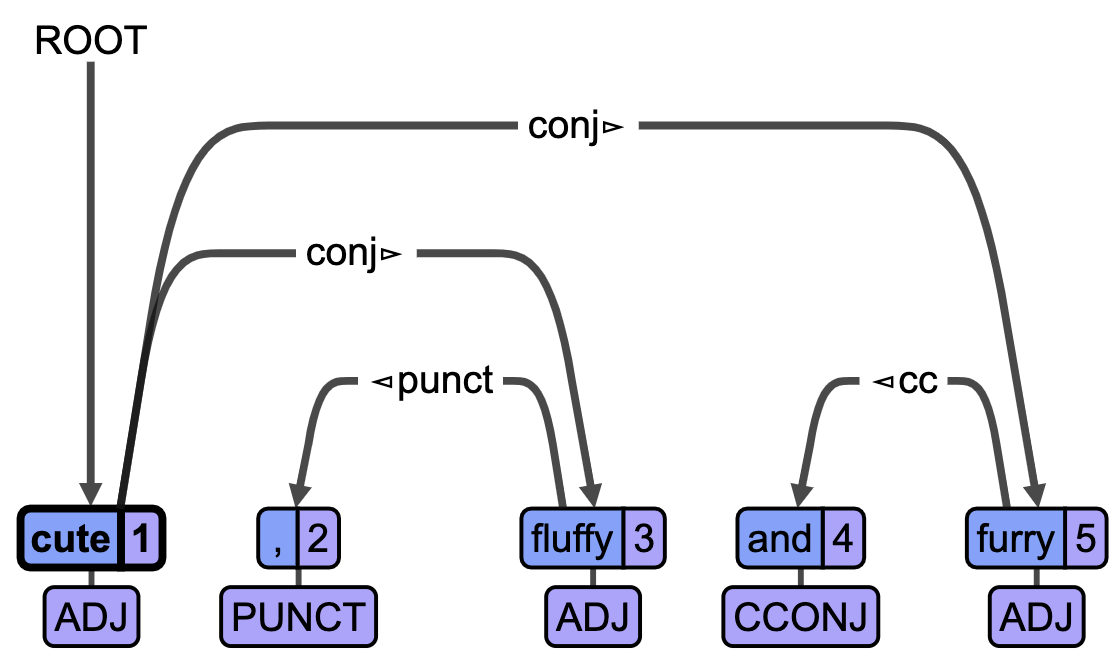
\includegraphics[width=0.7\textwidth]{figure/ud_cute.png}
    \begin{dependency}
        \begin{deptext}[column sep=0.4cm]
              small \& , \& furry \&  , \& fluffy \& and \& cute \\
            {\tt ADJ}\&{\tt PUNCT}\&{\tt ADJ}\&{\tt PUNCT}\&{\tt ADJ}\&{\tt CCONJ}\&{\tt ADJ}\\
        \end{deptext}
        \depedge{3}{2}{punct}
        \depedge{1}{3}{conj}
        \depedge{5}{4}{punct}
        \depedge{1}{5}{conj}
        \depedge{7}{6}{cc}
        \depedge{1}{7}{conj}
    \end{dependency} \\
    \caption{The phrase ``small, furry, fluffy and cute'' as a UD tree in graphical format}
    \label{fig:ud_cute}
\end{figure}
% \include{}

\begin{figure}
    \centering
    % \begin{dependency}
  \begin{deptext}[column sep=0.4cm]
      cute \& , \& fluffy \& and \& furry \\
    {\tt ADJ}\&{\tt PUNCT}\&{\tt ADJ}\&{\tt CCONJ}\&{\tt ADJ} \\
  \end{deptext}
  \depedge{2}{1}{punct}
  \depedge{0}{2}{conj}
  \depedge{4}{3}{cc}
  \depedge{0}{4}{conj}
\end{dependency} \\
    % \includesvg{ud-annotatrix-corpus.svg}
    % 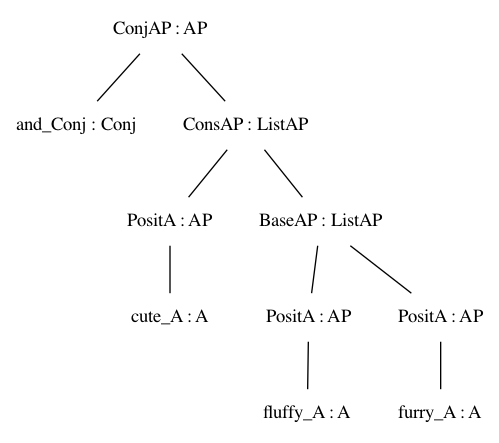
\includegraphics[width=0.7\textwidth]{figure/cute_gf.png}
    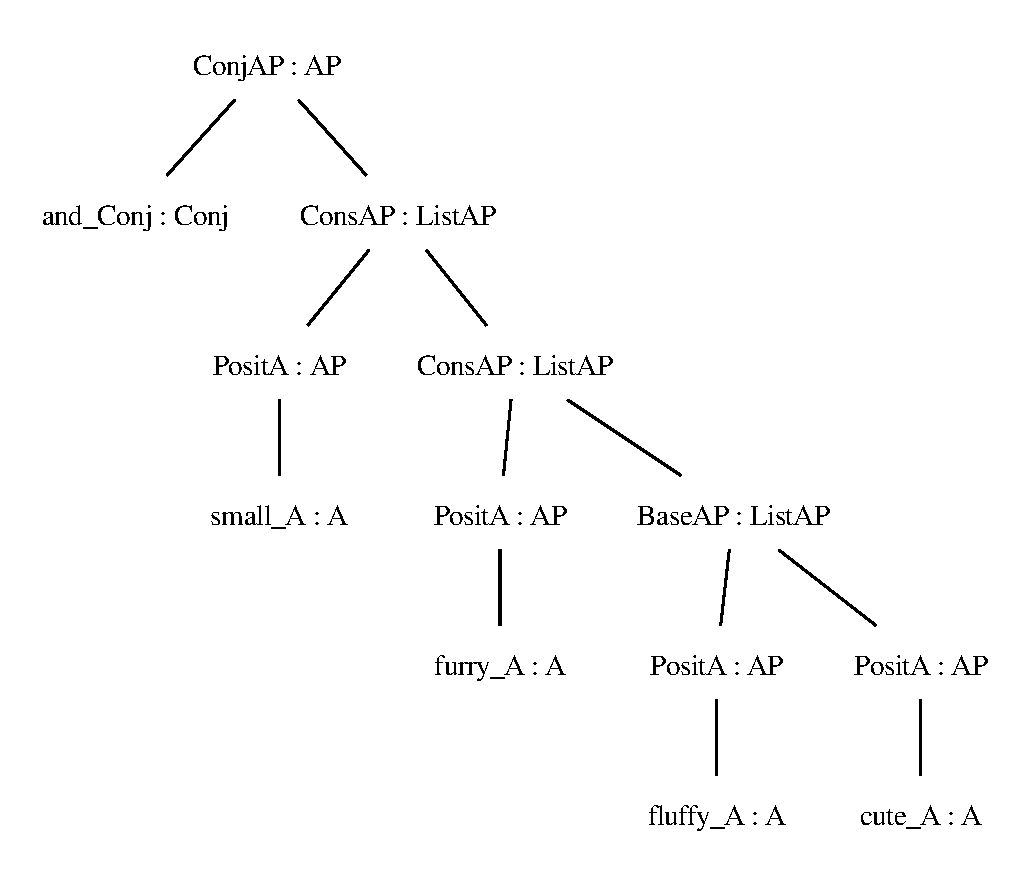
\includegraphics[width=0.7\textwidth]{figure/cute_gf.eps}
    % Generated with
    % vt -format=eps ConjAP and_Conj (ConsAP (PositA small_A) (ConsAP (PositA furry_A) (BaseAP (PositA fluffy_A) (PositA cute_A))))
    % on the UDApp.pgf grammar
    \caption{The phrase ``small, furry, fluffy and cute'' as a GF tree in graphical format. }
    \label{fig:gf_cute}
\end{figure}

The GF version of the same tree, shown in Figure \ref{fig:gf_cute}, would look like this:

\begin{verbatim}
ConjAP and_Conj (ConsAP (PositA cute_A)
                        (BaseAP (PositA fluffy_A) (PositA furry_A)))
\end{verbatim}
Here we can see that in UD, the word ``cute'' is in the root, while the conjunction ``and'' is at the bottom of the tree, while in GF the conjunction is a direct child of the root. This transformation can not be preformed by the simple single-layer transformations that are available in the current macro-system for labels files.

The main issue that made it impossible for the old macros to perform this transformation is that we need to extract several pieces of information from a node and then use them independently

\section{Solution: Recursive macros}

% Most of the time the structure in UD trees are similar enough to allow a fairly direct translation.
% There are however some difficult cases where the structure is significantly different in a way that was impossible to overcome using the old macro system.
%
% One such example is when you have a series of conjunctions, for example the phrase:
%
%
%   small, fluffy, furry and cute
%
% In

In order to improve the ability to create structurally different trees when converting from UD to GF, the ability for macros to be recursive was added.
This means that when a macro is substituted, the resulting head is checked again to see if the result is another macro, until no more substitutions are possible.
This makes it possible to encode data using Church-encoding, in particular the church encoding for pairs: a higher order function that takes a binary function as an argument and provides the two items it contains to the inner function.
This construction of pairs can also be interpreted as continuation-passing style, where instead of constructing a pair, we take a continuation which would consume the two arguments of the pair.

\begin{verbatim}
type Pair a b = forall c. (a -> b -> c) -> c
\end{verbatim}

In order to construct and consume these pairs we use the following helper functions:
\begin{lstlisting}
-- ab2r = a -> b -> r
-- Pair_a_b = ab2r -> r
#auxfun MkPair_ a b handler : a -> b -> ab2r -> r = handler a b ; head dummy dummy
#auxfun UsePair_ handler pair : ab2r -> Pair_a_b -> r = pair handler ; head dummy
\end{lstlisting}
The \verb|UsePair_| helper is not strictly necessary, since it can be replaced with function application, but it helps making the code clearer.

When using these helpers, you would partially apply the \verb|MkPair_| helper, so it can later get the final \verb|handler| argument from \verb|UsePair_|.

% \begin{lstlisting}
% #auxfun AndCuteCont_ and cute : Conj -> AP -> Pair_Conj_AP = MkPair_ and cute ; cc head
% \end{lstlisting}

In addition to pairs, we will also need triples, which work similarly:
\begin{lstlisting}
-- Triple_a_b_c = (a -> b -> r) -> r
#auxfun MkTriple_ a b c handler : a -> b -> c -> abc2r -> r = handler a b c ; head dummy nonexistent nope
#auxfun UseTriple_ handler triple : abc2r -> Triple_a_b_c -> r = triple handler ; head dummy
\end{lstlisting}

As can be seen in \autoref{fig:ud_cute}, each word but the first and last in a coordinate structure has a comma as a dependent in UD. This macro handles that.
\begin{lstlisting}
#auxfun CommaAP_ ap comma : AP -> Conj -> APComma =  ap ; head punct[LEMMA=\,]
\end{lstlisting}

The last word has the conjunction as a child in UD, while the conjunction is inserted at the very top in the GF syntax, as can be seen in \autoref{fig:gf_cute}. This is where we first use our \verb|MkPair_| helper in order to carry along the last word and the conjunction separately.
\begin{lstlisting}
#auxfun AndCuteCont_ and cute : Conj -> AP -> Pair_Conj_AP = MkPair_ and cute ; cc head
\end{lstlisting}
% TODO: Make names here match the figure
% TODO: Maybe make a larger picture

% Here we have the case
The simplest case is when we only have two words with a conjunction in between (``small and cute'').
The two functions below handles this case.
We need to handle this case separately because lists in GF have a minimum length of two.

We need a separate \verb|AP2_helper_| function to handle the extra argument \texttt{small} because we don't have support for lambdas or closures. We can see that the main function \verb|AP2_| gets both parts of the pair ``and cute'' as a bundle, while the \verb|AP2_helper_| gets them as separate arguments. Because the helper is only used by other macros, we don't need any real dependency labels but instead use dummy values to fill them in (here \texttt{dummy} and \texttt{nonexistent}, but anything would work).
\begin{lstlisting}
#auxfun AP2_ small andCute : AP -> Pair_Conj_AP -> AP = UsePair_ (AP2_helper_ small) andCute ; head conj
#auxfun AP2_helper_ small and cute :  AP -> Conj -> AP -> AP = ConjAP and (BaseAP small cute) ; head dummy nonexistent
\end{lstlisting}

The next case is when we have at least three content words with a conjunction (``small, fluffy and cute''). Here we need to create a triple, with:
\begin{itemize}
    \item the first word in the coordination, which is also the head of the UD tree (``small'')
    \item the conjunction (``and'')
    \item the two last content words (``fluffy'' and ``cute'') which form base of the GF list (\verb|BaseAP fluffy cute|).
\end{itemize}
\begin{lstlisting}
#auxfun APBaseComma_ small fluffy andCute : AP -> APComma -> Pair_Conj_AP -> ConjListAP = UsePair_ (APBaseComma_helper_ small fluffy) andCute ; head conj conj
#auxfun APBaseComma_helper_ small fluffy and cute : AP -> APComma -> Conj -> AP -> ConjListAP = MkTriple_ and small (BaseAP fluffy cute) ; head dummy dummy
\end{lstlisting}

The next case is for four or more content words with a conjunction (``small, furry, fluffy and cute''). Here we deconstruct the triple, add the middle word (``furry'') to the list (\verb|ConsAP furry (BaseAP fluffy cute)|) and reconstruct the triple.
\begin{lstlisting}
#auxfun APAddComma_ furry and_small_fluffyCute  : APComma -> ConjListAP -> ConjListAP = UseTriple_ (APAddComma_helper_ furry) and_small_fluffyCute ; conj head
#auxfun APAddComma_helper_ furry and small fluffyCute : APComma -> Conj -> AP -> ListAP -> ConjListAP = MkTriple_ and small (ConsAP furry fluffyCute) ; dummy head
\end{lstlisting}

Finally, we have can take a complete list and convert it into an adjectival phrase (AP). We deconstruct the triple of: a conjunction (``and''), first content word (``small'') and list of the remaining content words (``furry'', ``fluffy'', ``cute''
%: \verb|ConsAP furry (BaseAP fluffy cute)|
) and construct the final coordinate structure: \verb|ConjAP and (ConsAP small furryFluffyCute)| to arrive at the GF tree that can be seen in \autoref{fig:gf_cute}.
\begin{lstlisting}
#auxfun ConjListToAP2_ and_small_furryFluffyCute : ConjListAP -> AP = UseTriple_ ConjListToAP2_helper_ and_small_furryFluffyCute ; head
#auxfun ConjListToAP2_helper_ and small furryFluffyCute : Conj -> AP -> ListAP -> AP = ConjAP and (ConsAP small furryFluffyCute) ; notreal head dummy
\end{lstlisting}

The complete code of conjunctions using recursive macros can be seen in \autoref{appendix:conjunctions}.

% I am totally lost here. The explanations doesn't tell me anything and the appendix is just a source code dump. For some reason some of the functions are also commented out which makes me wonder whether these are alternative implementations or unsuccessful attempts.
%
% Ok. You use continuation passing style which makes it possible to return two things at once. At some point you need to go from continuation passing to normal function applications. How do you see that you have consumed all conjuncts and it is time to switch back?
%
% Good idea but I need to reconstruct the solution myself.  I suggest that you move the appendix here and comment on the different parts.


% \subsection{Evaluation example}

% The macros are expanded in a top-down fashion

\section{Limitations and ideas for further improvements}

A more structured implementation of this could be to add (anonymous) records as well as pattern matching to the syntax of macros similar to the concrete syntax of GF. A suggestion for how it could look can be seen commented out in \autoref{appendix:conjunctions}.

It could also be useful to have a more direct approach for describing the structural changes, especially since macros are only available in the \texttt{ud2gf} direction, not in the \texttt{gf2ud} direction.
